%%%%%%%%%%%%%%%%%%%%%%%%%%%%%%%%%%%%%%%%%
% baposter Portrait Poster
% LaTeX Template
% Version 1.0 (15/5/13)
%
% Created by:
% Brian Amberg (baposter@brian-amberg.de)
%
% This template has been downloaded from:
% http://www.LaTeXTemplates.com
%
% License:
% CC BY-NC-SA 3.0 (http://creativecommons.org/licenses/by-nc-sa/3.0/)
%
%%%%%%%%%%%%%%%%%%%%%%%%%%%%%%%%%%%%%%%%%

%----------------------------------------------------------------------------------------
%	PACKAGES AND OTHER DOCUMENT CONFIGURATIONS
%----------------------------------------------------------------------------------------

\documentclass[a0paper,portrait]{baposter}

\usepackage[font=small,labelfont=bf]{caption} % Required for specifying captions to tables and figures
\usepackage{booktabs} % Horizontal rules in tables
\usepackage{relsize} % Used for making text smaller in some places

\graphicspath{{figures/}} % Directory in which figures are stored

\definecolor{bordercol}{RGB}{40,40,40} % Border color of content boxes
\definecolor{headercol}{RGB}{186,215,230} % Background color for the header in the content boxes (left side)
\definecolor{headerfontcol}{RGB}{0,0,0} % Text color for the header text in the content boxes
\definecolor{boxcolor}{RGB}{255,255,255} % Background color for the content in the content boxes

\begin{document}

\begin{poster}{
grid=false,
%columns=1,
borderColor=bordercol, % Border color of content boxes
headerColorOne=headercol, % Background color for the header in the content boxes (left side)
headerColorTwo=headercol, % Background color for the header in the content boxes (right side)
headerFontColor=headerfontcol, % Text color for the header text in the content boxes
boxColorOne=boxcolor, % Background color for the content in the content boxes
headershape=roundedright, % Specify the rounded corner in the content box headers
headerfont=\Large\sf\bf, % Font modifiers for the text in the content box headers
textborder=rectangle,
background=none,
headerborder=open, % Change to closed for a line under the content box headers
boxshade=plain
}
{}
%
%----------------------------------------------------------------------------------------
%	TITLE AND AUTHOR NAME
%----------------------------------------------------------------------------------------
%
{\sf\bf PFS Software Infrastructure at Subaru} % Poster title
{\vspace{1em} Craig Loomis, Eiji Kyono and Hassan Siddiqui\\ % Author names
{\smaller cloomis@astro.princeton.edu, kyono@naoj.org, hassans@astro.princeton.edu}} % Author email addresses
{
% The logos are compressed a bit into a simple box to make them smaller on the result
% (Wasn't able to find any bigger of them.)
\setlength\fboxsep{0pt}
\setlength\fboxrule{0.5pt}
	\fbox{
		\begin{minipage}{14em}
			
\includegraphics[width=10em,height=4em]{PU-standard} 
			
\includegraphics[width=4em,height=4em]{subaru_color1_2400}
		\end{minipage}
	}
}

%----------------------------------------------------------------------------------------
%	INTRODUCTION
%----------------------------------------------------------------------------------------

\headerbox{Introduction}{name=introduction,column=0,row=0, span=3}{
The PFS software installed at Subaru needs to process and store critical science and calibration data during the course of operations. 
The infrastructure on which the software runs must therefore be robust and reliable. 
This poster outlines the current infrastructure in place, open issues and future plans.
}

%----------------------------------------------------------------------------------------
%	TARGET INFRASTRUCTURE
%----------------------------------------------------------------------------------------

\headerbox{Target Infrastructure}{name=infra,column=0, span=3, below=introduction}{

Currently there are 2 hosts and 1 NFS machine processing data during the MCS engineering runs in April and Oct 2018. This will be extended to target infrastructure below. 
This consists of 3 hosts and two NFS boxes to provide as much redundancy and flexibility as possible. 

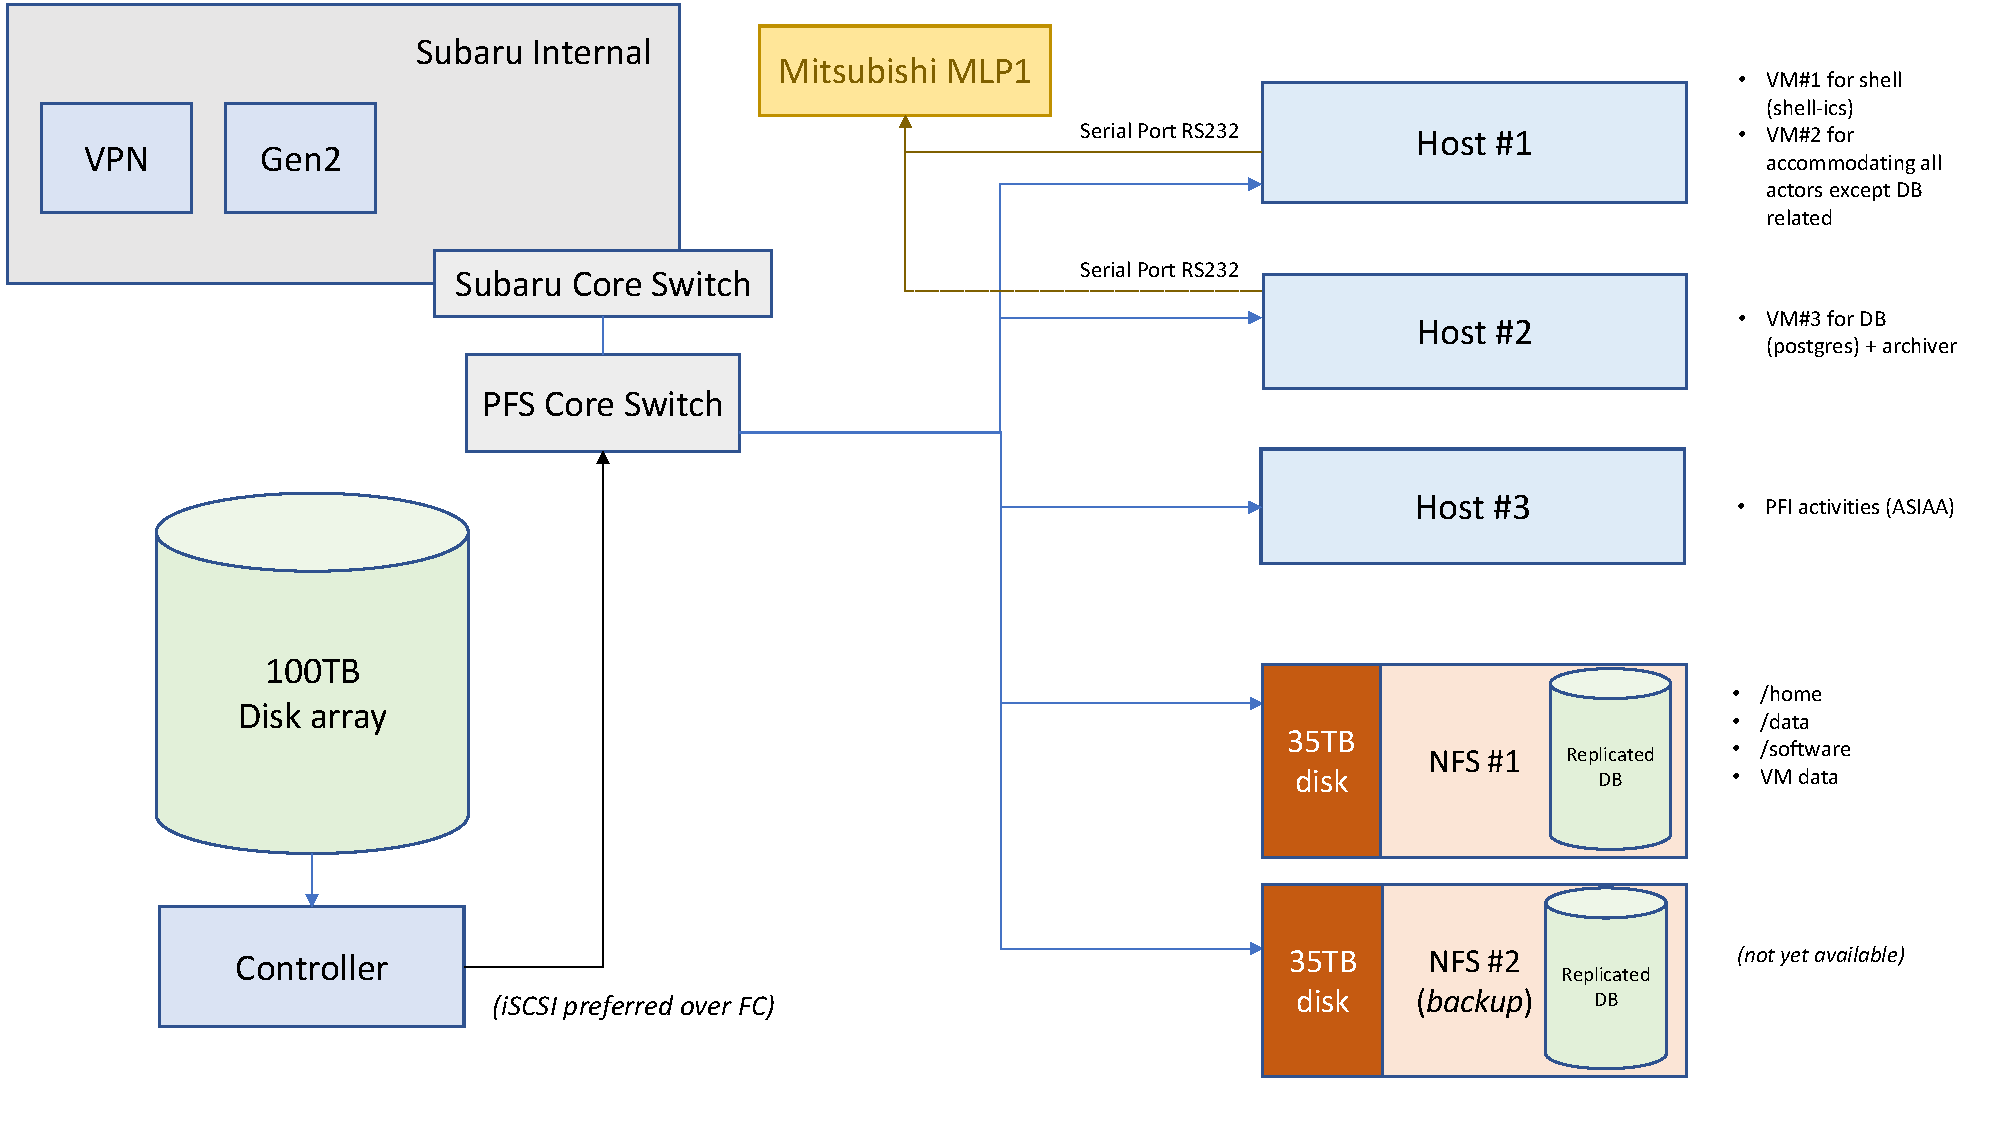
\includegraphics[width=0.9\linewidth]{PfsIcsMhsHardwareConfigTarget}
}

%----------------------------------------------------------------------------------------
%	CORE SWITCH LAYOUT
%----------------------------------------------------------------------------------------

\headerbox{Core Switch Layout}{name=switches,column=0, span=2, below=infra}{

The detailed core switch configuration and ethernet connections to the host and NFS machines are shown below.

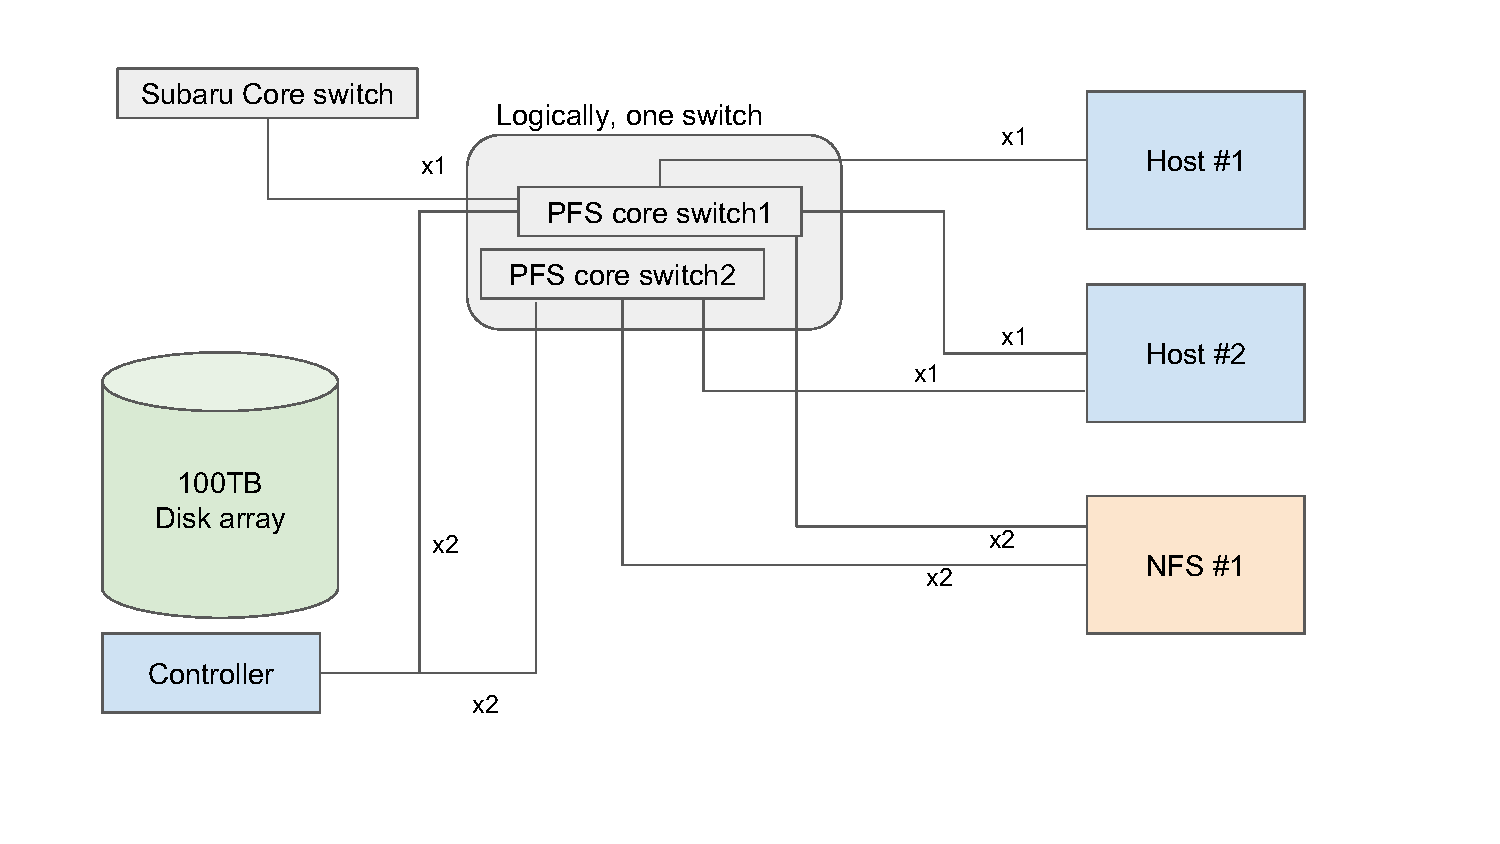
\includegraphics[width=0.9\linewidth]{DetailP2_Eth}
}


%----------------------------------------------------------------------------------------
%	OPEN POINTS
%----------------------------------------------------------------------------------------

\headerbox{Open Points}{name=plans,column=2,below=infra, bottomaligned=switches}{

\begin{enumerate}
\item The 35TB (physical size=60TB; effective capacity=35TB) disk arrays on NFS-1 and -2 are still to be confirmed, pending on the number of slots available and the cost.
\item The NFS-2 machine still needs to be purchased. How is the responsible (Subaru or PFS) is to be discussed.
\item iSCSI links are preferred over fiber cable. It is felt that the former are more robust. This may introduce a performance penalty however.
\end{enumerate}
}

%----------------------------------------------------------------------------------------
%	ACKNOWLEDGEMENTS
%----------------------------------------------------------------------------------------

\headerbox{Acknowledgements}{name=acknowledgements,column=0, span=3, below=switches}{
\begin{enumerate}
\item H.S. and C.L. acknowledge support by the National Science Foundation under Grant No 1636426 and support from the NAOJ.
\end{enumerate}
}

%-------------
% END
%-------------
\end{poster}

\end{document}
